%%%%%%%%%%%%%%%%%%%%
%% KAPITEL ANHANG %%
%%%%%%%%%%%%%%%%%%%%
\section{HANA Beispieldaten}

\lstset{language=SQL, caption={Beispieldaten anlegen \cite{SAPSCN}}, label={anhang:hanasql}}								
\begin{lstlisting}
CREATE COLUMN TABLE "SALES_F" ("SALES_ORDER_NBR" BIGINT CS_FIXED NOT NULL ,
       "CALENDAR_DAY" DAYDATE CS_DAYDATE,
       "BUSINESS_UNIT_ID" BIGINT CS_FIXED,
       "MATERIAL_ID" BIGINT CS_FIXED,
       "SUPPLIER_ID" BIGINT CS_FIXED,
       "UNIT_PRICE" DOUBLE CS_DOUBLE,
       "QUANTITY_SOLD" DOUBLE CS_DOUBLE,
       PRIMARY KEY ("SALES_ORDER_NBR"));

CREATE COLUMN TABLE "BUSINESS_UNIT_D" ("BUSINESS_UNIT_ID" BIGINT CS_FIXED NOT NULL ,
       "BUSINESS_UNIT_CODE" NVARCHAR(5),
       "BUSINESS_UNIT_DESC" NVARCHAR(256),
       "PARENT_BUSINESS_UNIT_ID" BIGINT CS_FIXED,
       "PARENT_BUSINESS_UNIT_CODE" NVARCHAR(5),
       PRIMARY KEY ("BUSINESS_UNIT_ID"));

CREATE COLUMN TABLE "SUPPLIER_D" ("SUPPLIER_ID" BIGINT CS_FIXED,
       "SUPPLIER_DESC" VARCHAR(60),
       PRIMARY KEY("SUPPLIER_ID"));

CREATE COLUMN TABLE "MATERIAL_D" ("MATERIAL_ID" BIGINT CS_FIXED,
       "SKU" VARCHAR(16),
       "MATERIAL_GROUP" VARCHAR(60),
       PRIMARY KEY("MATERIAL_ID"));
 
INSERT INTO "BUSINESS_UNIT_D"
VALUES(1,'BU1','Business Unit 1',0,'');
INSERT INTO "BUSINESS_UNIT_D"
VALUES(2,'BU2','Business Unit 2',1,'BU1');
INSERT INTO "BUSINESS_UNIT_D"
VALUES(3,'BU3','Business Unit 3',1,'BU1');
INSERT INTO "BUSINESS_UNIT_D"
VALUES(4,'BU4','Business Unit 4',2,'BU2');
INSERT INTO "BUSINESS_UNIT_D"
VALUES(5,'BU5','Business Unit 5',3,'BU3');
INSERT INTO "BUSINESS_UNIT_D"
VALUES(6,'BU6','Business Unit 6',3,'BU4');
INSERT INTO "BUSINESS_UNIT_D"
VALUES(7,'BU7','Business Unit 7',4,'BU4');
INSERT INTO "BUSINESS_UNIT_D"
VALUES(8,'BU8','Business Unit 6',4,'BU4');
 
CREATE COLUMN TABLE ADJECTIVE (ID INTEGER, WORD VARCHAR(60), PRIMARY KEY ("ID"));
CREATE COLUMN TABLE NOUN (ID INTEGER, WORD VARCHAR(60), PRIMARY KEY ("ID"));
CREATE COLUMN TABLE SUP_TYPE (ID INTEGER, WORD VARCHAR(60), PRIMARY KEY ("ID"));
 
INSERT INTO ADJECTIVE VALUES(1, 'Great');
INSERT INTO ADJECTIVE VALUES(2, 'Modern');
INSERT INTO ADJECTIVE VALUES(3, 'Fast');
INSERT INTO ADJECTIVE VALUES(4, 'Proud');
INSERT INTO ADJECTIVE VALUES(5, 'Solid');
INSERT INTO ADJECTIVE VALUES(6, 'Broad');
INSERT INTO ADJECTIVE VALUES(7, 'Elegant');
INSERT INTO ADJECTIVE VALUES(8, 'Fancy');
INSERT INTO ADJECTIVE VALUES(9, 'Mysterious');
INSERT INTO ADJECTIVE VALUES(10, 'Fantastic');
 
INSERT INTO NOUN VALUES(1, 'Factory');
INSERT INTO NOUN VALUES(2, 'Offices');
INSERT INTO NOUN VALUES(3, 'Industry');
INSERT INTO NOUN VALUES(4, 'Station');
INSERT INTO NOUN VALUES(5, 'Restaurant');
INSERT INTO NOUN VALUES(6, 'Buildings');
INSERT INTO NOUN VALUES(7, 'Mall');
INSERT INTO NOUN VALUES(8, 'Studio');
INSERT INTO NOUN VALUES(9, 'Stockbrokers');
INSERT INTO NOUN VALUES(10, 'Academy');
 
INSERT INTO SUP_TYPE VALUES(1, 'Limited');
INSERT INTO SUP_TYPE VALUES(2, 'Pty Ltd');
INSERT INTO SUP_TYPE VALUES(3, 'Partnership');
INSERT INTO SUP_TYPE VALUES(4, 'Group');
INSERT INTO SUP_TYPE VALUES(5, 'Trust');
INSERT INTO SUP_TYPE VALUES(6, 'Collective');
INSERT INTO SUP_TYPE VALUES(7, 'Consortium');
INSERT INTO SUP_TYPE VALUES(8, 'Inc.');
INSERT INTO SUP_TYPE VALUES(9, 'Traders');
INSERT INTO SUP_TYPE VALUES(10, 'Franchise');
 
CREATE SEQUENCE seq START WITH 1;
 
CREATE PROCEDURE BUILD_SUPPLIER_TABLE (IN NMBR INT) LANGUAGE SQLSCRIPT AS
CNTR INTEGER;
BEGIN
CNTR := 0;
WHILE CNTR < :NMBR DO
INSERT INTO SUPPLIER_D
SELECT seq.NEXTVAL,
            (SELECT TOP 1 WORD FROM ADJECTIVE WHERE ID = SUBSTR(ROUND(RAND() * 9, 0 ),1,1) + 1 ORDER BY WORD)  || ' ' ||
            (SELECT TOP 1 WORD FROM NOUN WHERE ID = SUBSTR(ROUND(RAND() * 9, 0 ),1,1) + 1 ORDER BY WORD) ||  ' ' ||
            (SELECT TOP 1 WORD FROM SUP_TYPE WHERE ID = SUBSTR(ROUND(RAND() * 9, 0 ),1,1) + 1 ORDER BY WORD)  AS SUPDESC
FROM DUMMY;      
CNTR := CNTR + 1;
END WHILE;
END;
 
CALL BUILD_SUPPLIER_TABLE(1000);
 
CREATE COLUMN TABLE MAT_GROUP (ID INTEGER, WORD VARCHAR(60), PRIMARY KEY ("ID"));
INSERT INTO MAT_GROUP VALUES(1, 'Engine');
INSERT INTO MAT_GROUP VALUES(2, 'Exterior');
INSERT INTO MAT_GROUP VALUES(3, 'Interior');
INSERT INTO MAT_GROUP VALUES(4, 'Accesories');
INSERT INTO MAT_GROUP VALUES(5, 'Electrical');
INSERT INTO MAT_GROUP VALUES(6, 'Components');
INSERT INTO MAT_GROUP VALUES(7, 'Finishing');
INSERT INTO MAT_GROUP VALUES(8, 'Hydraulics');
INSERT INTO MAT_GROUP VALUES(9, 'Liquids');
INSERT INTO MAT_GROUP VALUES(10, 'Extras');
 
CREATE PROCEDURE BUILD_MAT_GROUP_TABLE (IN NMBR INT) LANGUAGE SQLSCRIPT AS
CNTR INTEGER;
BEGIN
CNTR := 0;
WHILE CNTR < :NMBR DO
INSERT INTO MATERIAL_D
SELECT :CNTR,
       'SKU' || LPAD(ROUND((RAND() * 1000000),0),7,'0000000') as SKU,
            (SELECT TOP 1 WORD FROM MAT_GROUP WHERE ID = SUBSTR(ROUND(RAND() * 9, 0 ),1,1) + 1 ORDER BY WORD)  AS MATERIAL
FROM DUMMY;      
CNTR := CNTR + 1;
END WHILE;
END;
 
CALL BUILD_MAT_GROUP_TABLE(10000);
 
CREATE PROCEDURE BUILD_FACT_TABLE (IN NMBR INT) LANGUAGE SQLSCRIPT AS
CNTR INTEGER;
BEGIN
CNTR := 0;
WHILE CNTR < :NMBR DO
INSERT INTO SALES_F
SELECT :CNTR,
       ADD_DAYS (TO_DATE ('2011-01-01', 'YYYY-MM-DD'), RAND() * 730),
         ROUND((RAND() * (SELECT COUNT(*) FROM BUSINESS_UNIT_D)), 0 ),
         ROUND((RAND() * (SELECT COUNT(*) FROM MATERIAL_D)), 0 ),
         ROUND((RAND() * (SELECT COUNT(*) FROM SUPPLIER_D)), 0 ),
         ROUND(RAND() * 1000,2),
         ROUND(RAND() * 100,0)
FROM DUMMY;      
CNTR := CNTR + 1;
END WHILE;
END;
 
CALL BUILD_FACT_TABLE(10000000);
\end{lstlisting}

\section{Screenshots zum Workflow Builder}
\begin{figure}[H]
	\begin{center}
	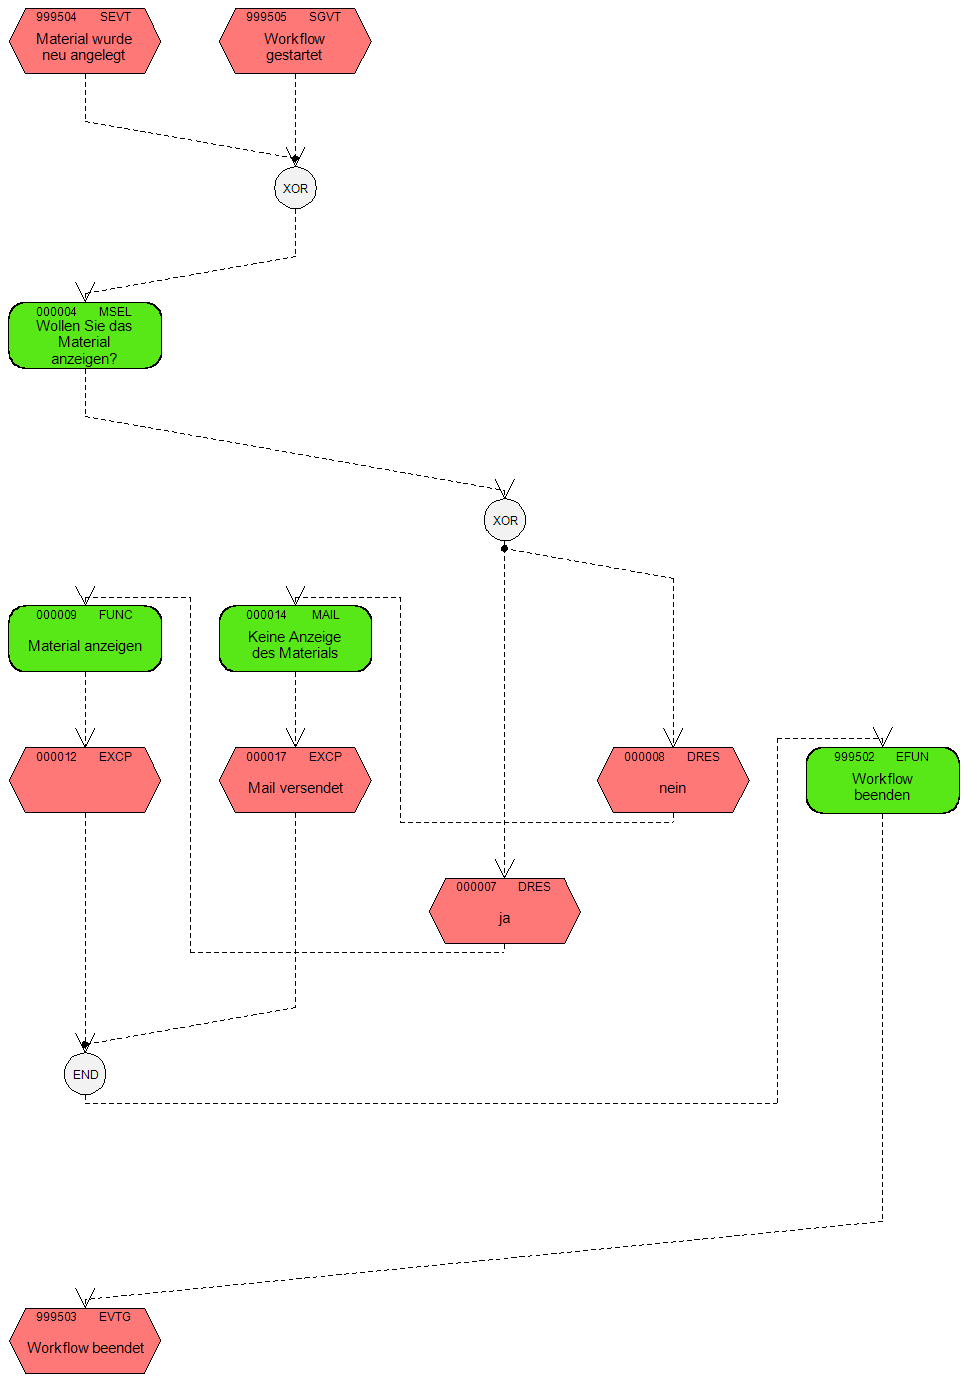
\includegraphics[height=0.9\textheight]{grafiken/wf-builder_view-classicepc.png}
	\caption{Ansicht eines Workflows als klassisches EPK}
	\vspace{-10pt}
	\label{abb:workflow-view-classicepc}
	\end{center}
\end{figure}

\begin{figure}[H]
	\begin{center}
	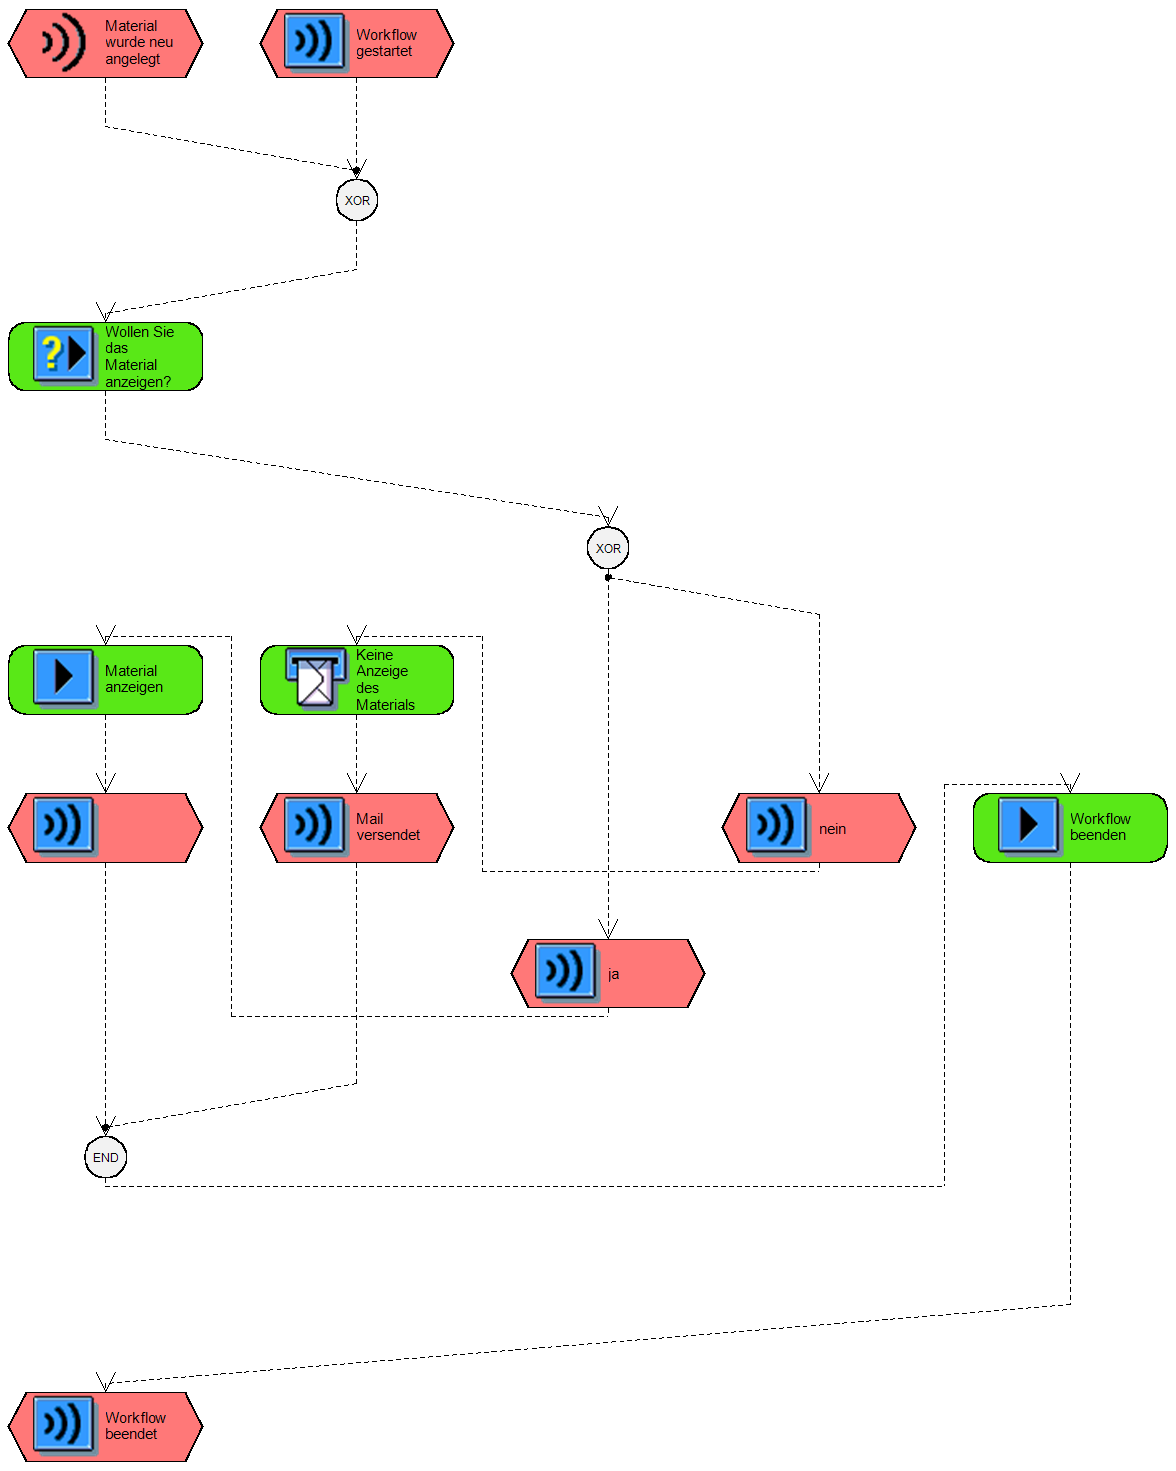
\includegraphics[width=1.0\textwidth]{grafiken/wf-builder_view-epc.png}
	\caption{Ansicht eines Workflows als Mischform beider Ansichten}
	\vspace{-10pt}
	\label{abb:workflow-view-epc}
	\end{center}
\end{figure}

\begin{figure}[H]
	\begin{center}
	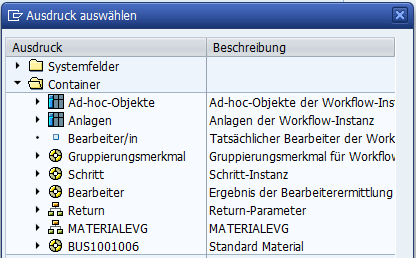
\includegraphics[width=250px]{grafiken/wf-builder_bsp1_formular-aufgabe_eingabehilfe-ausdruck.png}
	\caption{Eingabehilfe zum Ausdruck bei neuen Aufgaben}
	\vspace{-10pt}
	\label{abb:workflow-bsp1-aufgaben_form-inputhelp}
	\end{center}
\end{figure}

\begin{figure}[H]
	\begin{center}
	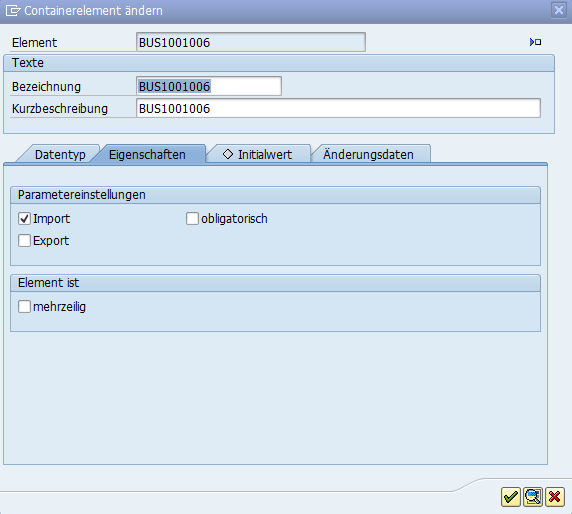
\includegraphics[width=350px]{grafiken/wf-builder_bsp1_formular-containerelement-edit.png}
	\caption{Einstellung zum Import eines Containerelements}
	\vspace{-10pt}
	\label{abb:workflow-bsp1-containeredit-import}
	\end{center}
\end{figure}

\begin{figure}[H]
	\begin{center}
	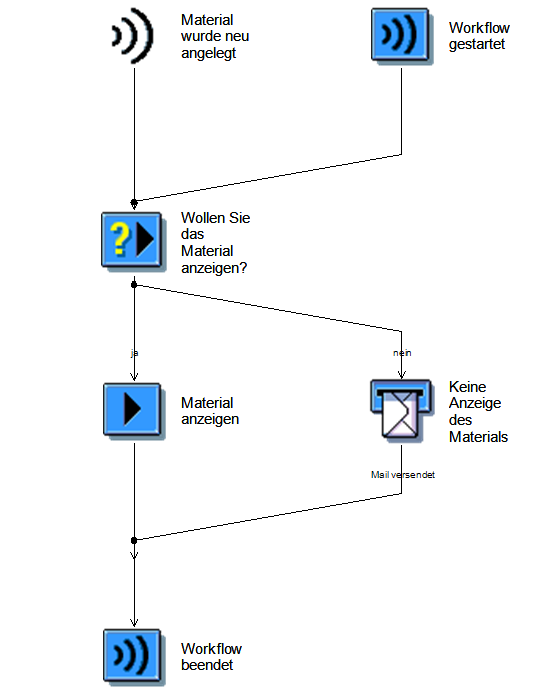
\includegraphics[height=0.7\textheight]{grafiken/wf-builder_bsp1_complete.png}
	\caption{Erster Beispielworkflow fertiggestellt}
	\vspace{-10pt}
	\label{abb:workflow-bsp1-complete}
	\end{center}
\end{figure}

\begin{figure}[H]
	\begin{center}
	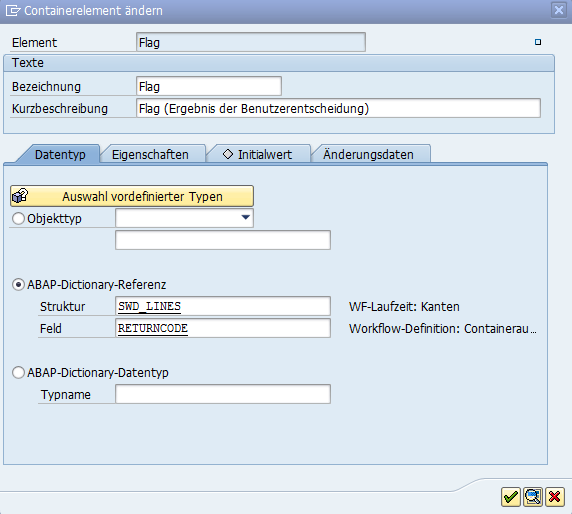
\includegraphics[height=400px]{grafiken/wf-builder_bsp2_container-flag.png}
	\caption{Konfiguration eines Containerelements als Flag}
	\vspace{-10pt}
	\label{abb:workflow-bsp2-container-flag}
	\end{center}
\end{figure}

\begin{figure}[H]
	\begin{center}
	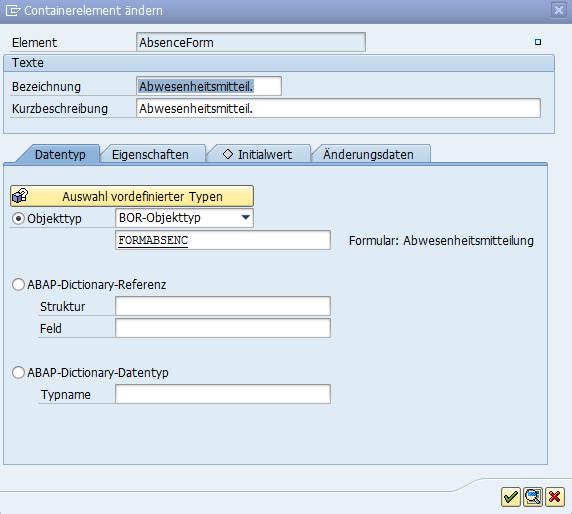
\includegraphics[height=400px]{grafiken/wf-builder_bsp2_container-form.png}
	\caption{Konfiguration eines Containerelements als Formular zur Abwesenheitsmitteilung}
	\vspace{-10pt}
	\label{abb:workflow-bsp2-container-form}
	\end{center}
\end{figure}

\begin{figure}[H]
	\begin{center}
	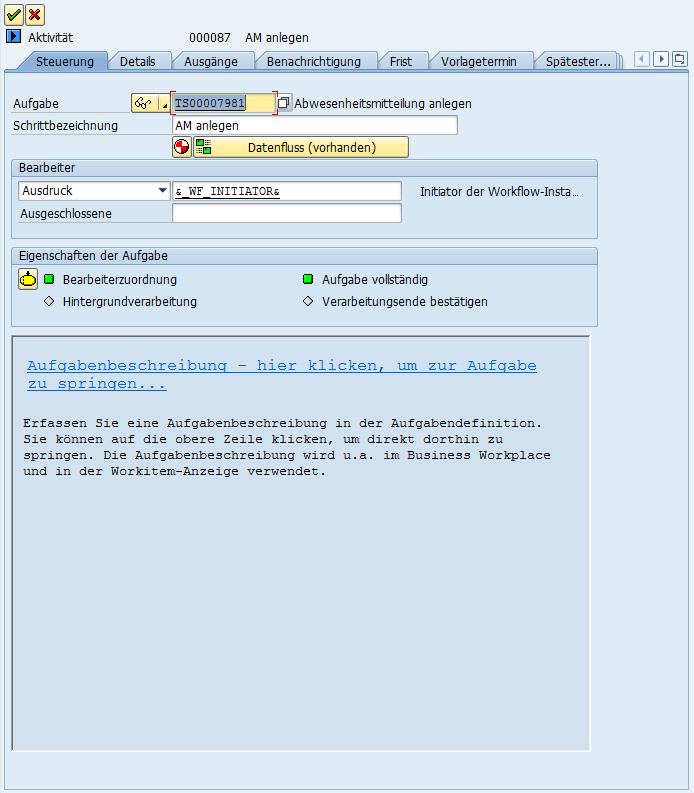
\includegraphics[width=1.0\textwidth]{grafiken/wf-builder_bsp2_act_am-anlegen.png}
	\caption{Konfiguration der Aufgabe Abwesenheitsmitteilung anlegen}
	\vspace{-10pt}
	\label{abb:workflow-bsp2-act_am-anlegen}
	\end{center}
\end{figure}

\begin{figure}[H]
	\begin{center}
	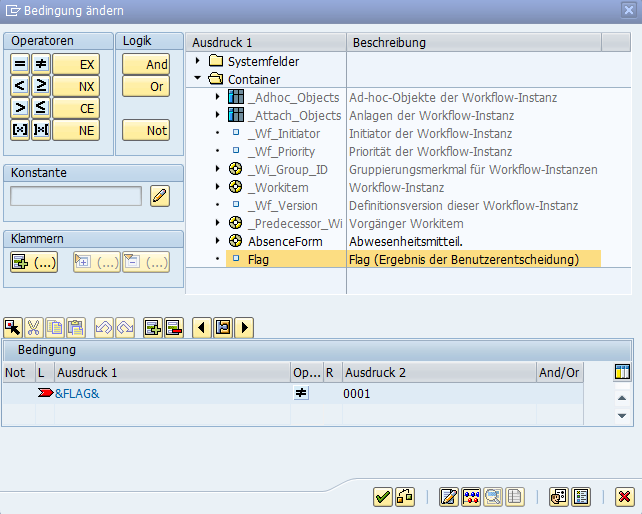
\includegraphics[width=450px]{grafiken/wf-builder_bsp2_act_loop_inputhelp.png}
	\caption{Eingabehilfe der Until-Schleife}
	\vspace{-10pt}
	\label{abb:workflow-bsp2-act_loop_inputhelp}
	\end{center}
\end{figure}

\begin{figure}[H]
	\begin{center}
	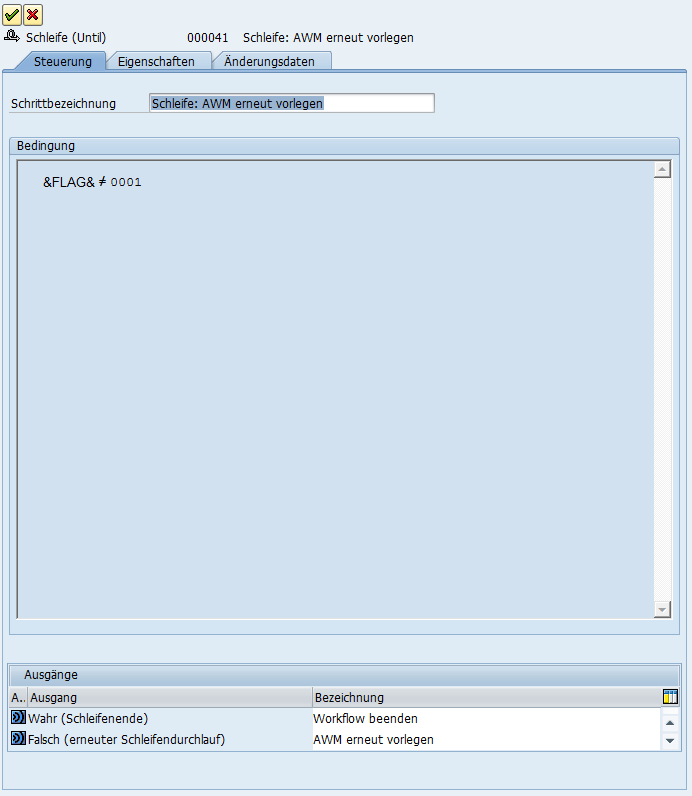
\includegraphics[width=1.0\textwidth]{grafiken/wf-builder_bsp2_act_loop.png}
	\caption{Konfiguration der Until-Schleife}
	\vspace{-10pt}
	\label{abb:workflow-bsp2-act_loop}
	\end{center}
\end{figure}

\begin{figure}[H]
	\begin{center}
	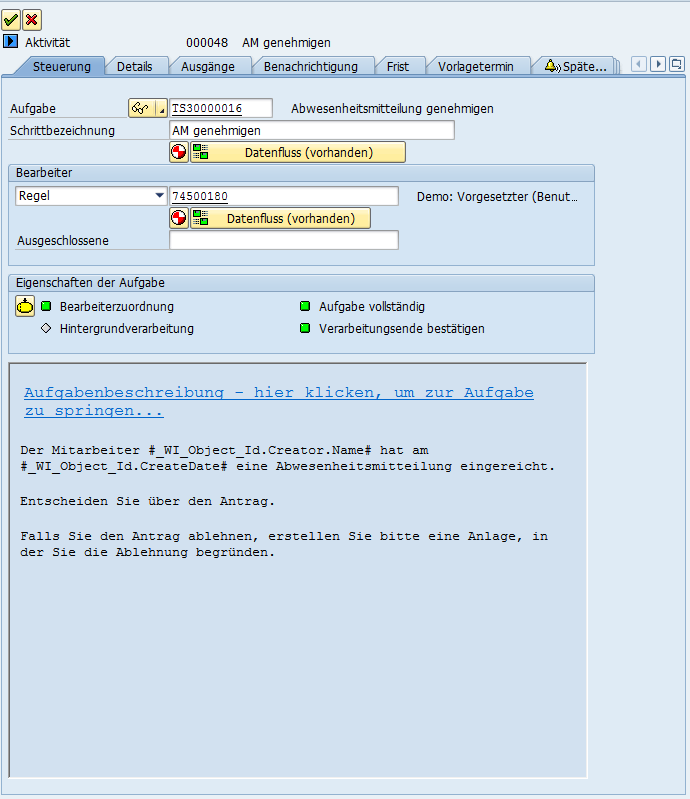
\includegraphics[width=1.0\textwidth]{grafiken/wf-builder_bsp2_act_am-genehmigen.png}
	\caption{Konfiguration der Aufgabe Abwesenheitsmitteilung genehmigen}
	\vspace{-10pt}
	\label{abb:workflow-bsp2-act_am-genehmigen}
	\end{center}
\end{figure}

\begin{figure}[H]
	\begin{center}
	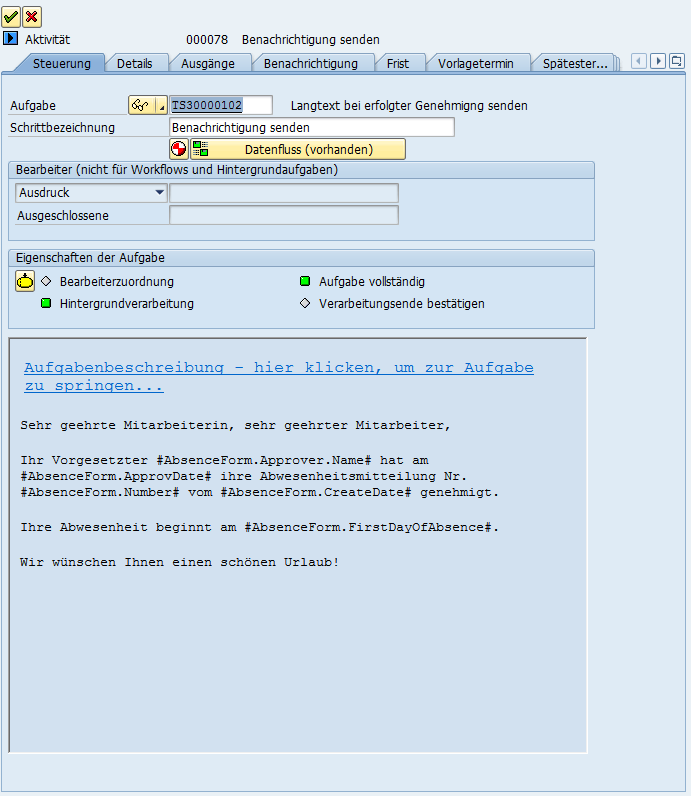
\includegraphics[width=1.0\textwidth]{grafiken/wf-builder_bsp2_act_message-genehmigt.png}
	\caption{Konfiguration der Aufgabe Benachrichtigung über Genehmigung}
	\vspace{-10pt}
	\label{abb:workflow-bsp2-act_message-genehmigt}
	\end{center}
\end{figure}

\begin{figure}[H]
	\begin{center}
	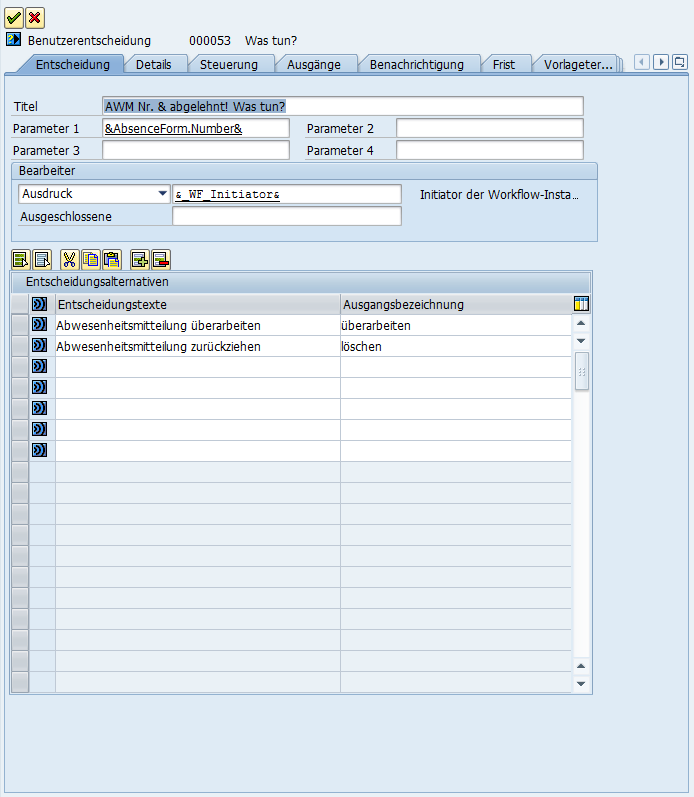
\includegraphics[width=1.0\textwidth]{grafiken/wf-builder_bsp2_act_was-tun.png}
	\caption{Konfiguration der Benutzerentscheidung nach Ablehnung}
	\vspace{-10pt}
	\label{abb:workflow-bsp2-act_was-tun}
	\end{center}
\end{figure}

\begin{figure}[H]
	\begin{center}
	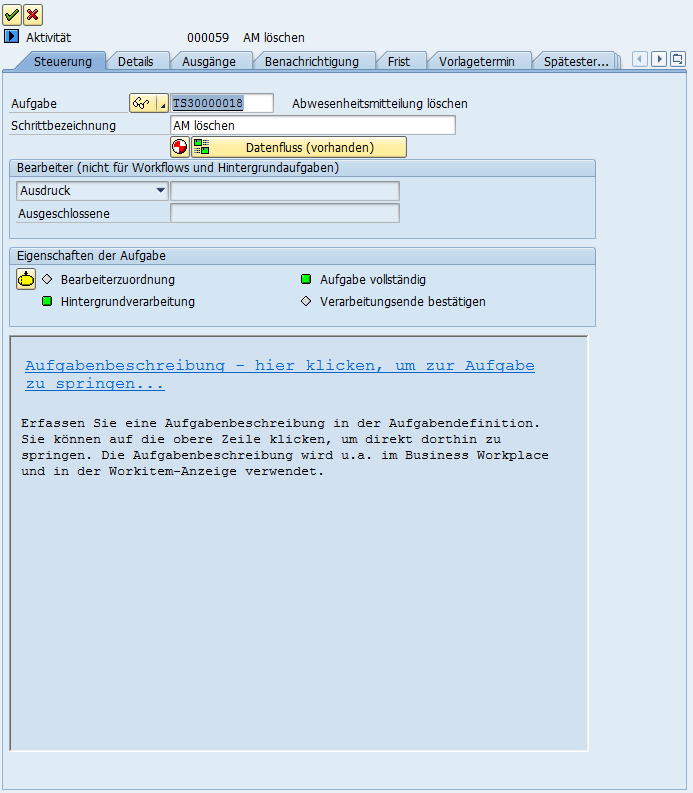
\includegraphics[width=1.0\textwidth]{grafiken/wf-builder_bsp2_act_am-loeschen.png}
	\caption{Konfiguration der Aufgabe zum Löschen einer Abwesenheitsmitteilung}
	\vspace{-10pt}
	\label{abb:workflow-bsp2-act_am-loeschen}
	\end{center}
\end{figure}

\begin{figure}[H]
	\begin{center}
	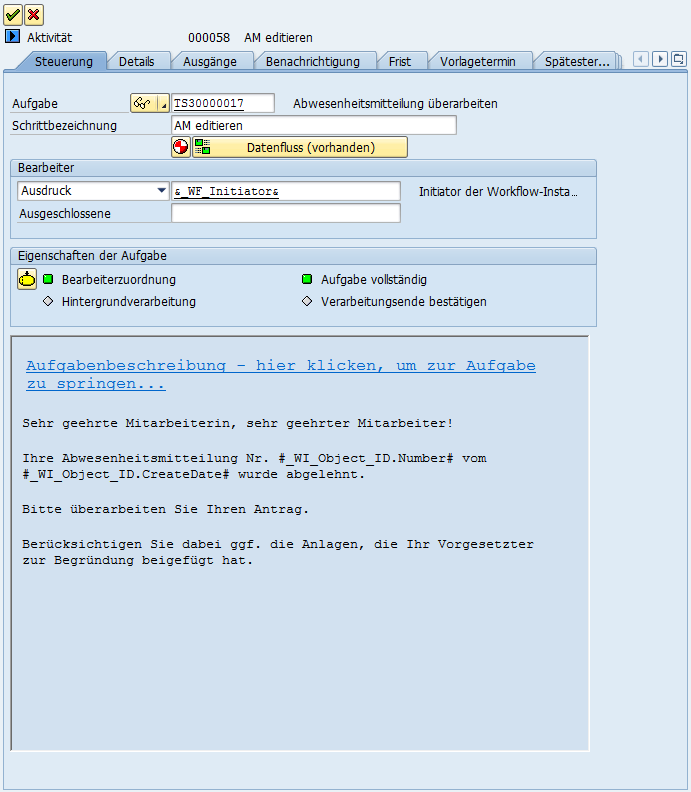
\includegraphics[width=1.0\textwidth]{grafiken/wf-builder_bsp2_act_am-editieren.png}
	\caption{Konfiguration der Aufgabe zum Editieren einer Abwesenheitsmitteilung}
	\vspace{-10pt}
	\label{abb:workflow-bsp2-act_am-editieren}
	\end{center}
\end{figure}

\begin{figure}[H]
	\begin{center}
	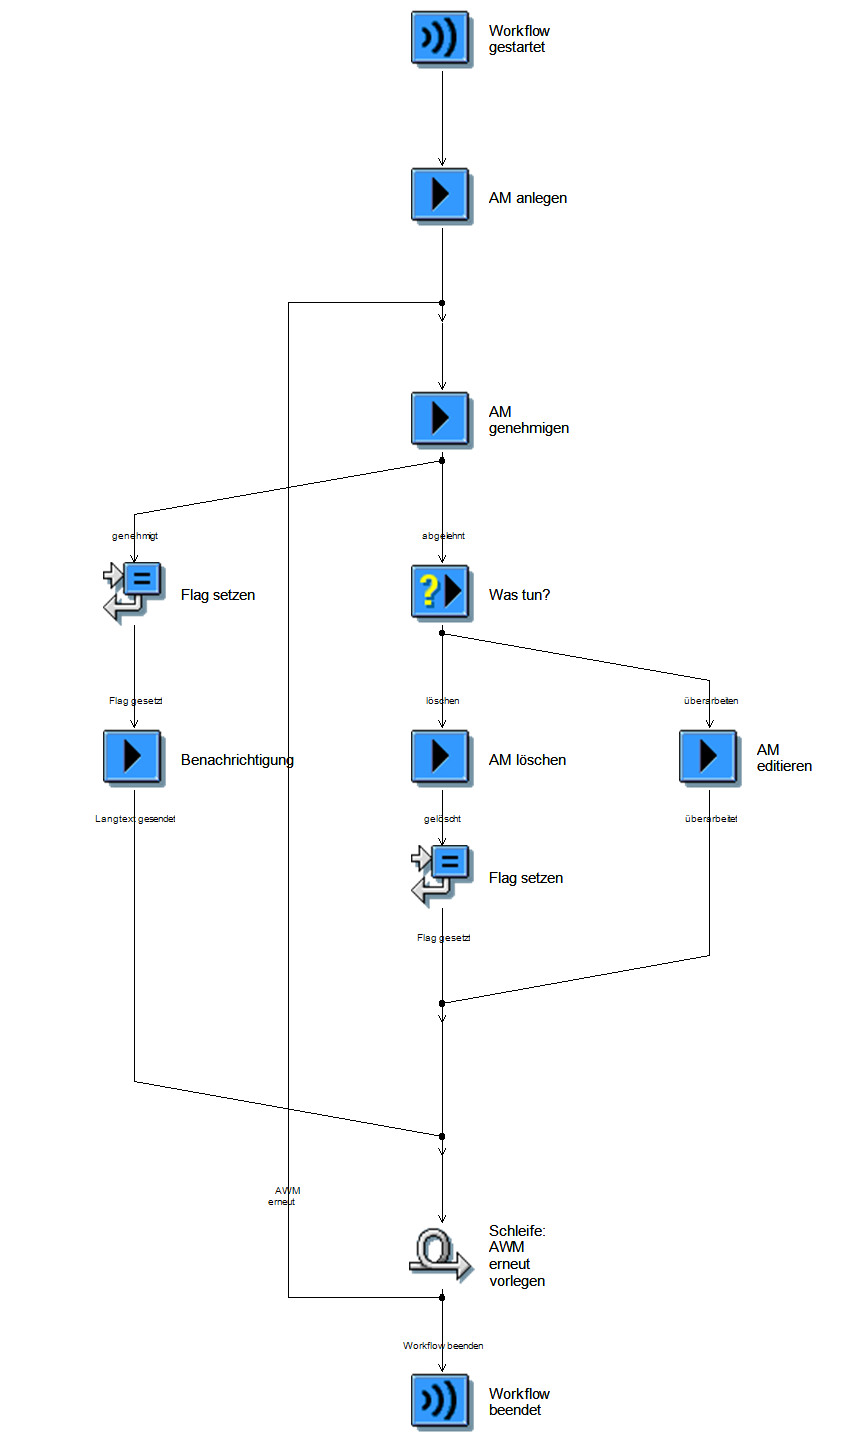
\includegraphics[height=0.95\textheight]{grafiken/wf-builder_bsp2_complete.png}
	\caption{Zweiter Beispielworkflow fertiggestellt}
	\vspace{-10pt}
	\label{abb:workflow-bsp2-complete}
	\end{center}
\end{figure}

\section{Business ByDesign Screenshots}

\begin{figure}[H]
	\begin{center}
	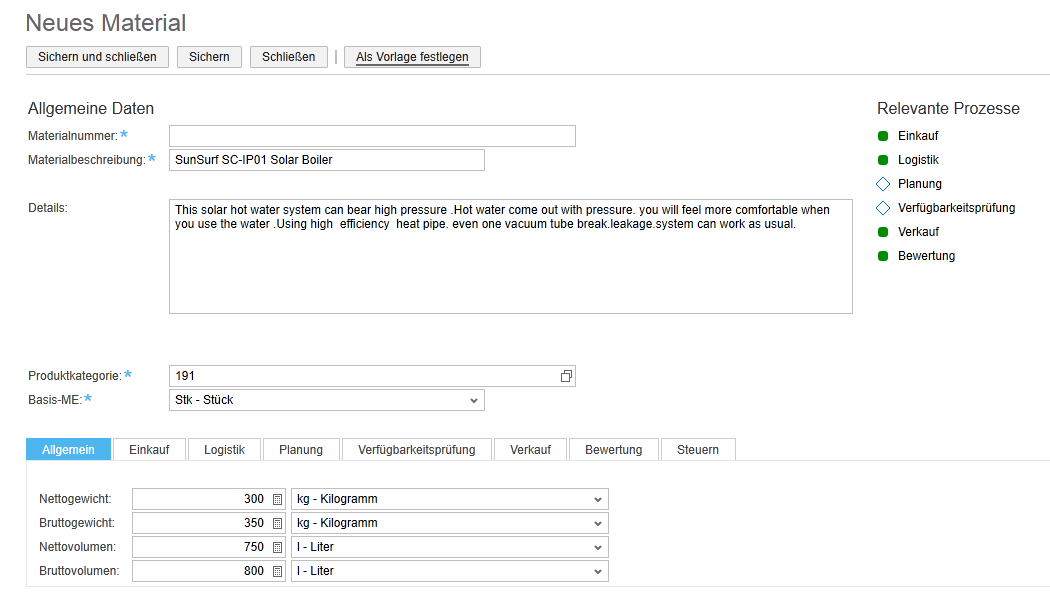
\includegraphics[width=1.0\textwidth]{grafiken/ByDesign-HowTo-1.png}
	\caption{Neues Material anlegen}
	\vspace{-10pt}
	\label{abb:byd-newmaterial}
	\end{center}
\end{figure}

\begin{figure}[H]
	\begin{center}
	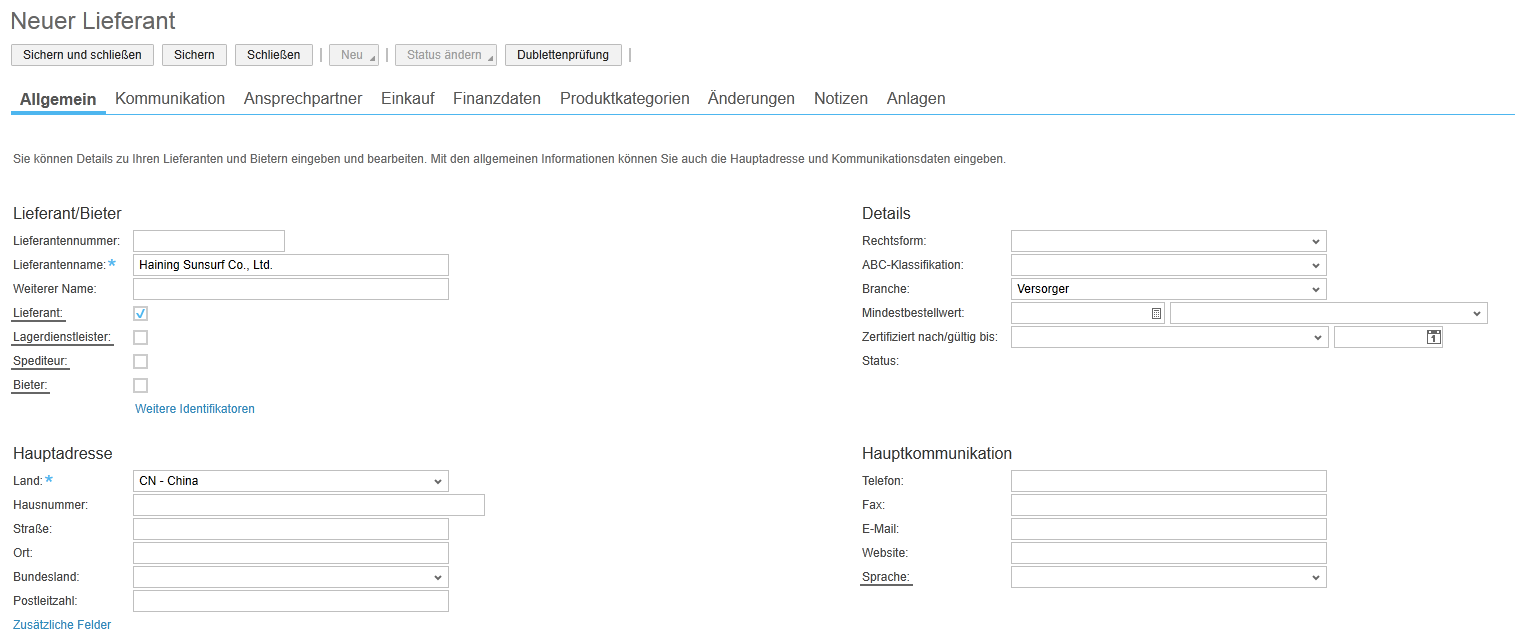
\includegraphics[width=1.0\textwidth]{grafiken/ByDesign-HowTo-2.png}
	\caption{Neuen Zulieferer anlegen}
	\vspace{-10pt}
	\label{abb:byd-newsupplier}
	\end{center}
\end{figure}

\begin{figure}[H]
	\begin{center}
	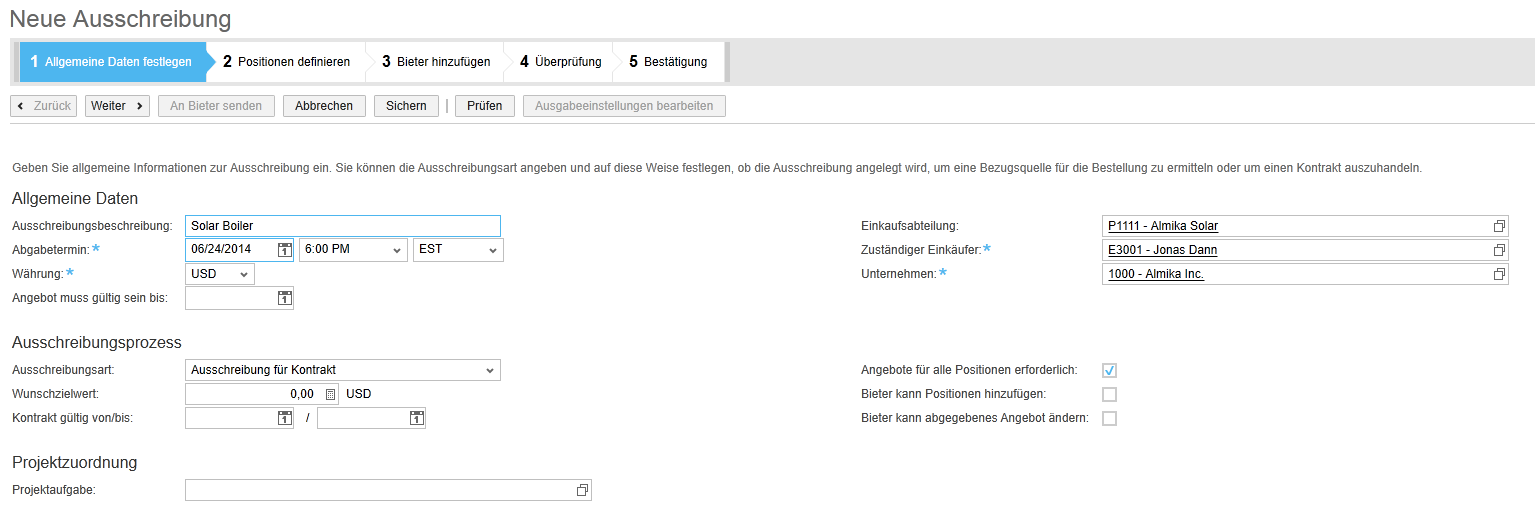
\includegraphics[width=1.0\textwidth]{grafiken/ByDesign-HowTo-Ausschreibung-1.png}
	\caption{Neue Ausschreibung erstellen - Allgemeine Daten}
	\vspace{-10pt}
	\label{abb:byd-rfq-1}
	\end{center}
\end{figure}

\begin{figure}[H]
	\begin{center}
	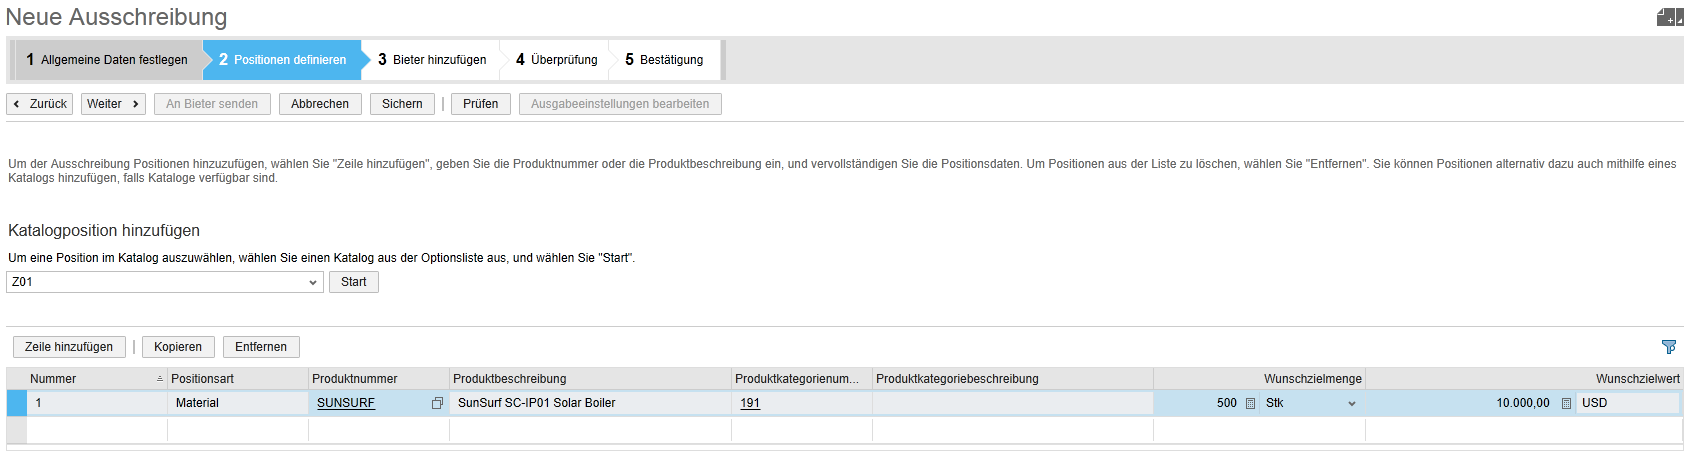
\includegraphics[width=1.0\textwidth]{grafiken/ByDesign-HowTo-Ausschreibung-2.png}
	\caption{Neue Ausschreibung erstellen - Positionen definieren}
	\vspace{-10pt}
	\label{abb:byd-rfq-2}
	\end{center}
\end{figure}

\begin{figure}[H]
	\begin{center}
	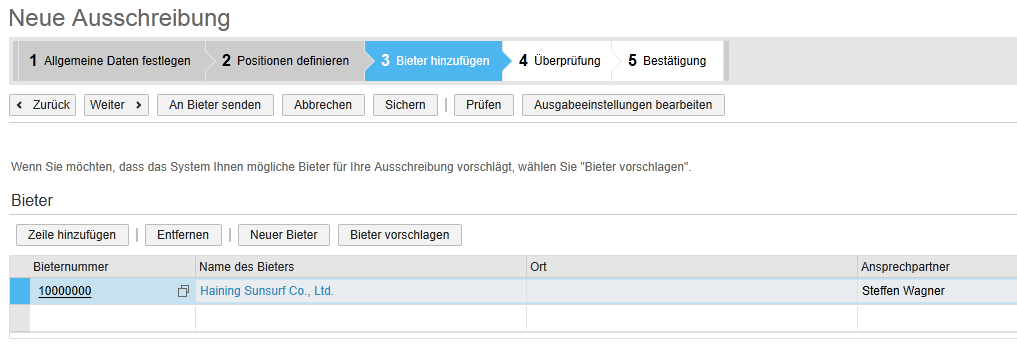
\includegraphics[width=1.0\textwidth]{grafiken/ByDesign-HowTo-Ausschreibung-3.png}
	\caption{Neue Ausschreibung erstellen - Bieter hinzufügen}
	\vspace{-10pt}
	\label{abb:byd-rfq-3}
	\end{center}
\end{figure}

\begin{figure}[H]
	\begin{center}
	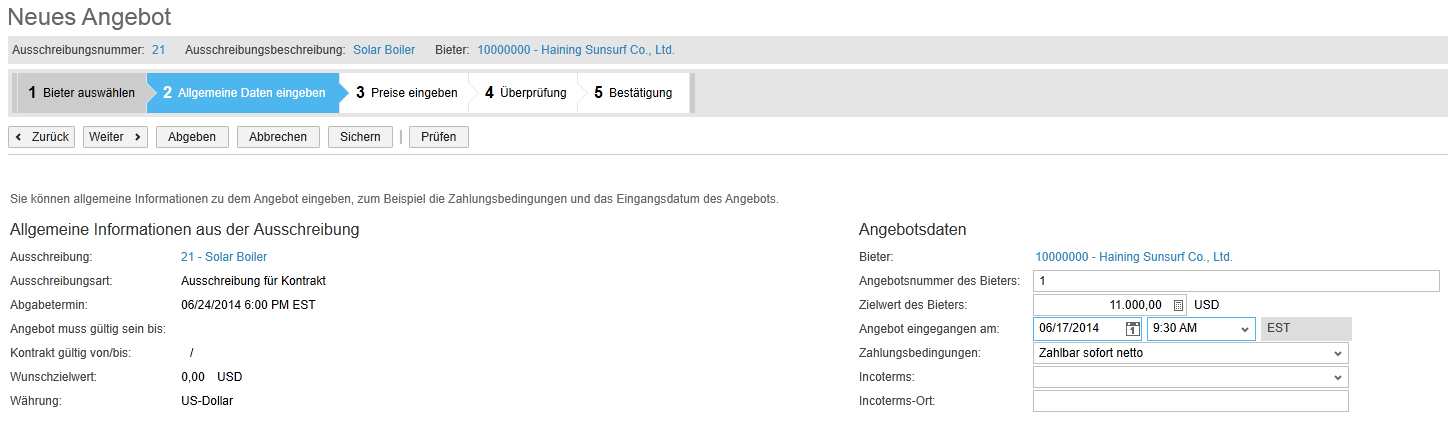
\includegraphics[width=1.0\textwidth]{grafiken/ByDesign-HowTo-Ausschreibung-4.png}
	\caption{Neues Angebot - Allgemeine Daten}
	\vspace{-10pt}
	\label{abb:byd-rfq-4}
	\end{center}
\end{figure}

\begin{figure}[H]
	\begin{center}
	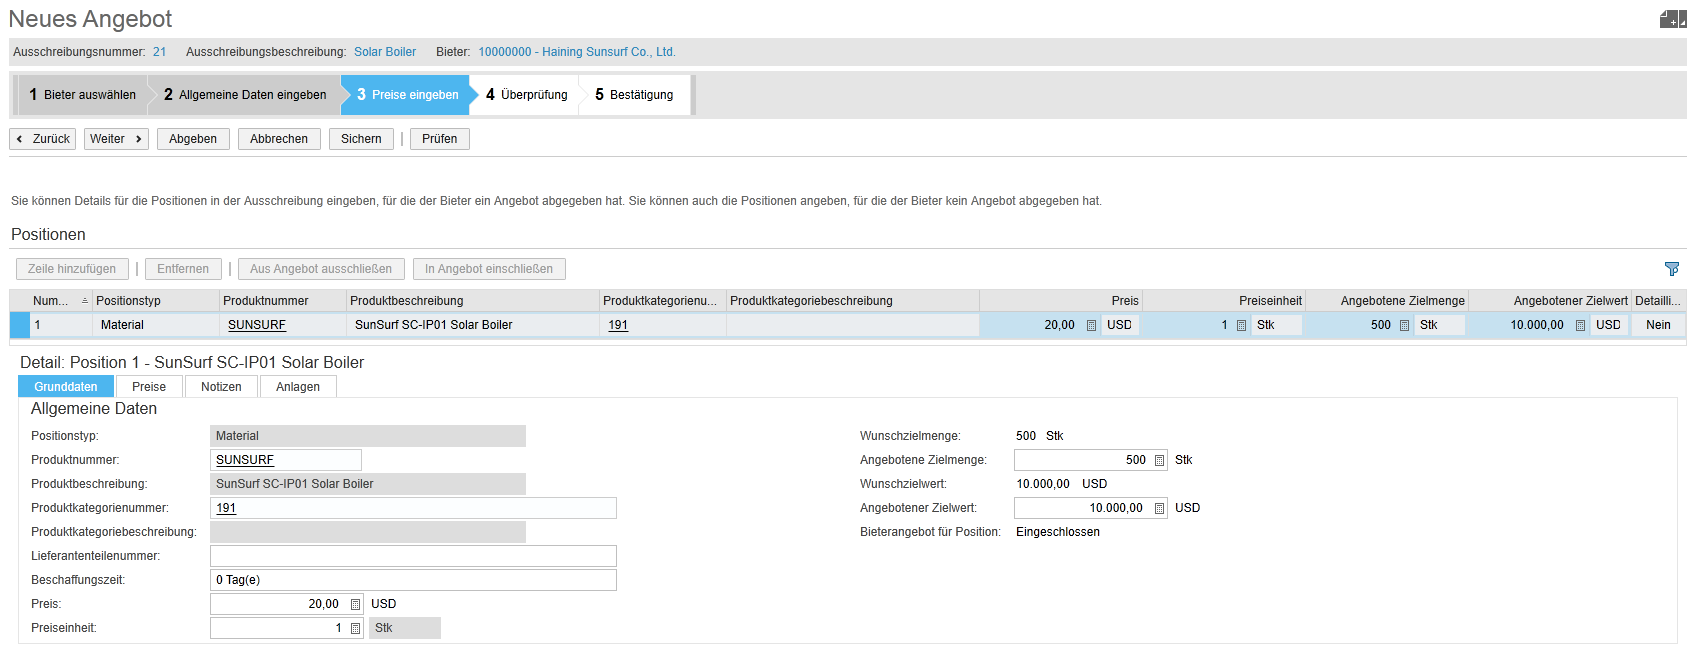
\includegraphics[width=1.0\textwidth]{grafiken/ByDesign-HowTo-Ausschreibung-5.png}
	\caption{Neues Angebot - Preise einfügen}
	\vspace{-10pt}
	\label{abb:byd-rfq-5}
	\end{center}
\end{figure}

\begin{figure}[H]
	\begin{center}
	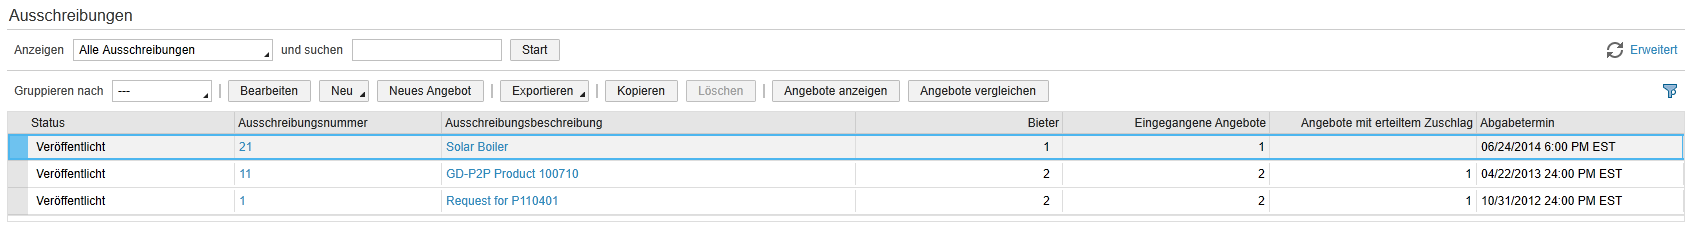
\includegraphics[width=1.0\textwidth]{grafiken/ByDesign-HowTo-Ausschreibung-6.png}
	\caption{Übersicht: Ausschreibungen}
	\vspace{-10pt}
	\label{abb:byd-rfq-6}
	\end{center}
\end{figure}

\begin{figure}[H]
	\begin{center}
	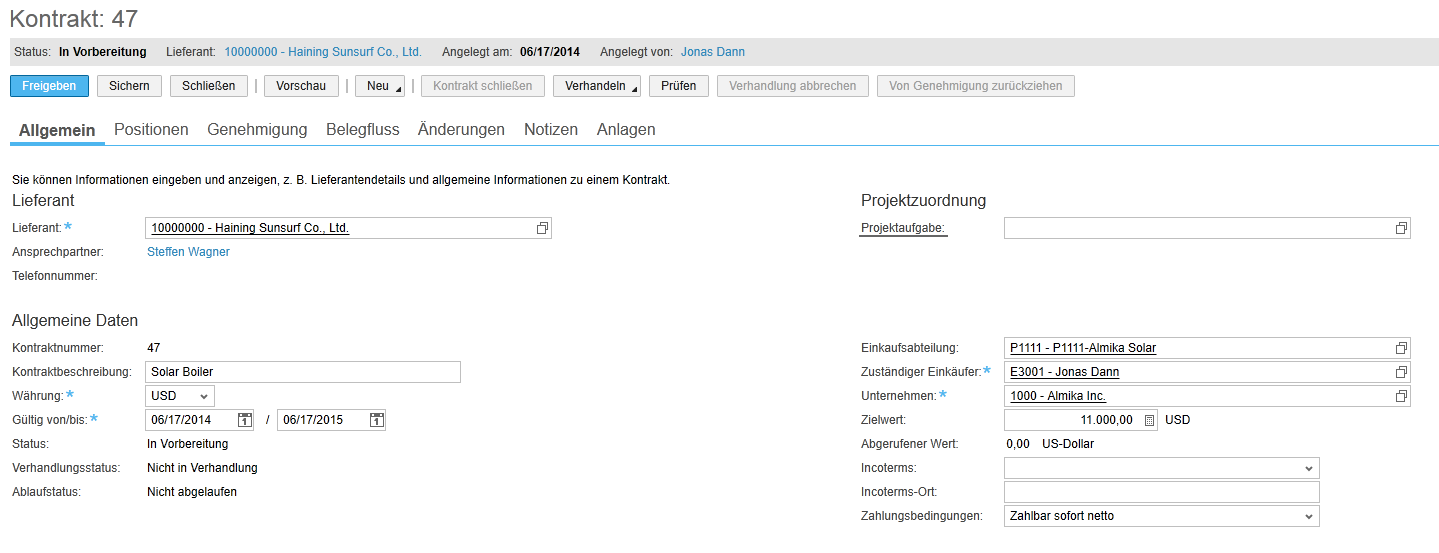
\includegraphics[width=1.0\textwidth]{grafiken/ByDesign-HowTo-4.png}
	\caption{Vertrag schließen}
	\vspace{-10pt}
	\label{abb:byd-contract}
	\end{center}
\end{figure}

\vspace{-10pt}